\documentclass[a4paper]{article}
\usepackage[utf8]{inputenc}
\usepackage{graphicx}
\usepackage{circuitikz}
\usepackage{placeins}
\usepackage{wrapfig}
\usepackage{siunitx}
\usepackage{hyperref}
\usepackage{epstopdf}
\usepackage{soul}
\usepackage{indentfirst}
\usepackage[margin=3cm]{geometry}

\title{Misura della Curva Caratteristica di una \\
Lampadina a Incandescenza}
\author{Giovanni Simionato \and Jia Le Sofia Zheng \and Francesco Giuliano Rossi}
\date{13 Ottobre 2025}


\begin{document}
\maketitle
\section{Introduzione}
In questa esperienza, si vuole misurare la curva caretteristica di una lampadina a incandescenza al variare del potenziale fino al bruciamento della stessa.

\begin{wrapfigure}{r}{0.5\textwidth}
\begin{circuitikz}\label{circuito}
   \draw (0,0) to[ battery1, name=myB ] (0,2)
   to [ resistor ] (3,2)
   to [ bulb ] (3,-1)
   to [ rmeter, t=A ] (0,-1)
   to (0,0)

   (2,1.5) to (3,1.5)
   (2,1.5) to [rmeter, t=V] (2,-0.5)
   to (3,-0.5)

   (4.3,2) to [photodiode, mirror] (4.3,-1)
   to (5.5,-1) 
   to [rmeter, t=V] (5.5,2)
   to (4.3,2);
   
   \ctikztunablearrow{1}{1}{60}{myB}
\end{circuitikz}
\caption{Circuito usato per $V<1$V}
\end{wrapfigure}
A questo scopo, si è costruito un circuito come in figura \ref{circuito}, dove la lampadina e il fotodiodo erano isolati dall'ambiente esterno da un tubo di plastica e nastro isolante nero. Il circuito sulla sinistra è costituito da un alimentatore da laboratorio, una resistenza da $100.4\pm0.1 \Omega$, una lampadina da 6V per 0.300A, e due multimetri. Il circuito sulla destra è costituito da un fotodiodo ad alimentazione interna collegato ad un multimetro. 

L'esperimento si è svolto in due fasi. Per tensioni al di sotto di un Volt, si sono tenuti connessi al circuito la resistenza e il fotodiodo. In questo modo si può rilevare il momento in cui la lampadina si illumina, misurando la corrente in uscita dal fotodiodo. La resistenza è stata usata per avere un controllo più fine sul potenziale ai capi della lampadina, dato che la manopola sull'alimentatore non permetteva di avere incrementi abbastanza fini. 
Nella seconda fase, si è scollegata la resistenza e si è tolto il fotodiodo. Il potenziale è stato portato ad un valore inferiore rispetto a quello più alto misurato nella prima fase e poi incrementato fino al bruciamento del filamento. 

\section{Dati Raccolti e Analisi}
Di seguito riportiamo tutti i dati raccolti in forma di grafico della corrente rispetto al potenziale.

%primo grafico e descrizione
\begin{figure}[!htbp] \label{fig2}
  \centering
      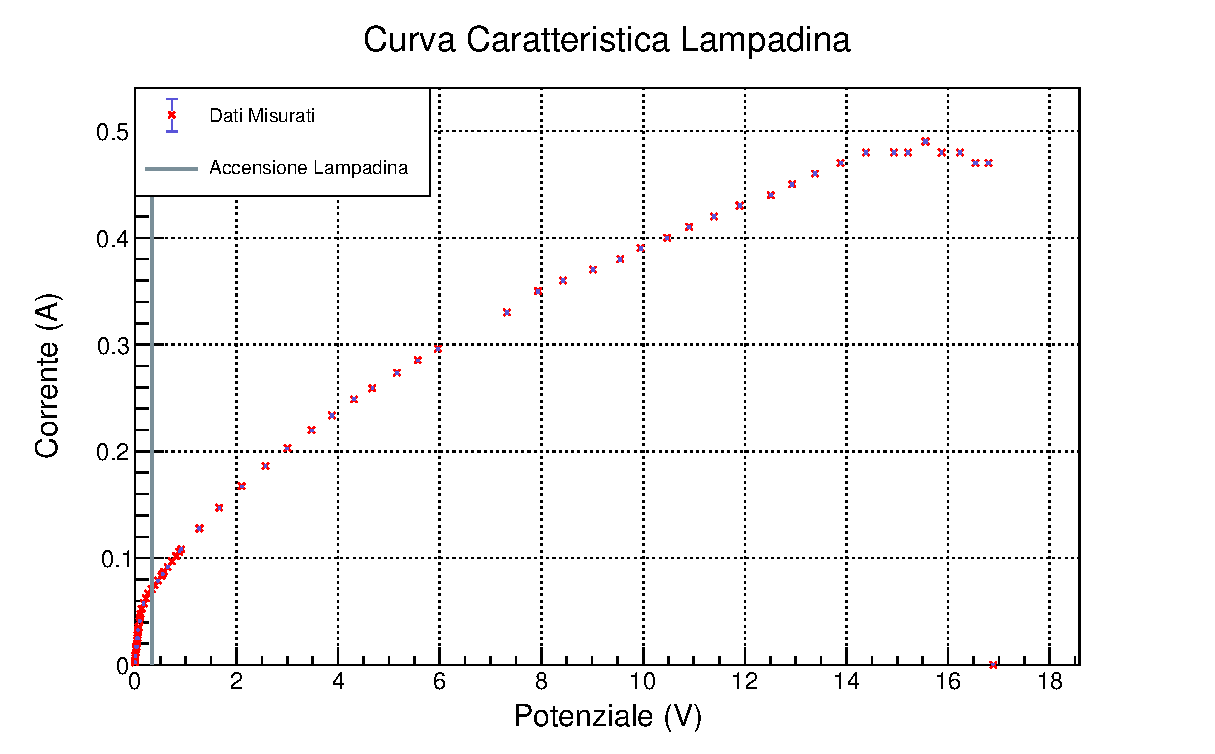
\includegraphics[width=0.9\textwidth]{immagini/bruciarelampa.eps}
        \caption{Curva caratteristica della lampadina a incandescenza}
\end{figure}
\FloatBarrier
Si può notare che all'inizio l'andamento è in buona approssimazione lineare (vedi Figura 3), come descritto dalla legge di Ohm. Il fit lineare ottenuto con il metodo dei minimi quadrati ha come equazione y=mx+q, con pendenza m=(0.4708$\pm 0.0002) \Omega$ e intercetta q$=(1.069\pm0.009)\times10^3$A.

Essendo un grafico della corrente rispetto al potenziale, la resistenza è uguale all'inverso della pendenza, che ci porta ad avere un valore della resistenza della lampadina di $(2.1242\pm 0.0009) \Omega$. Per il fit lineare, sono stati considerati dati fino a $V=0.0756$V, dato che dopo devia da un comportamento lineare. 

\begin{figure}[!htbp]\label{fig3}
  \centering
      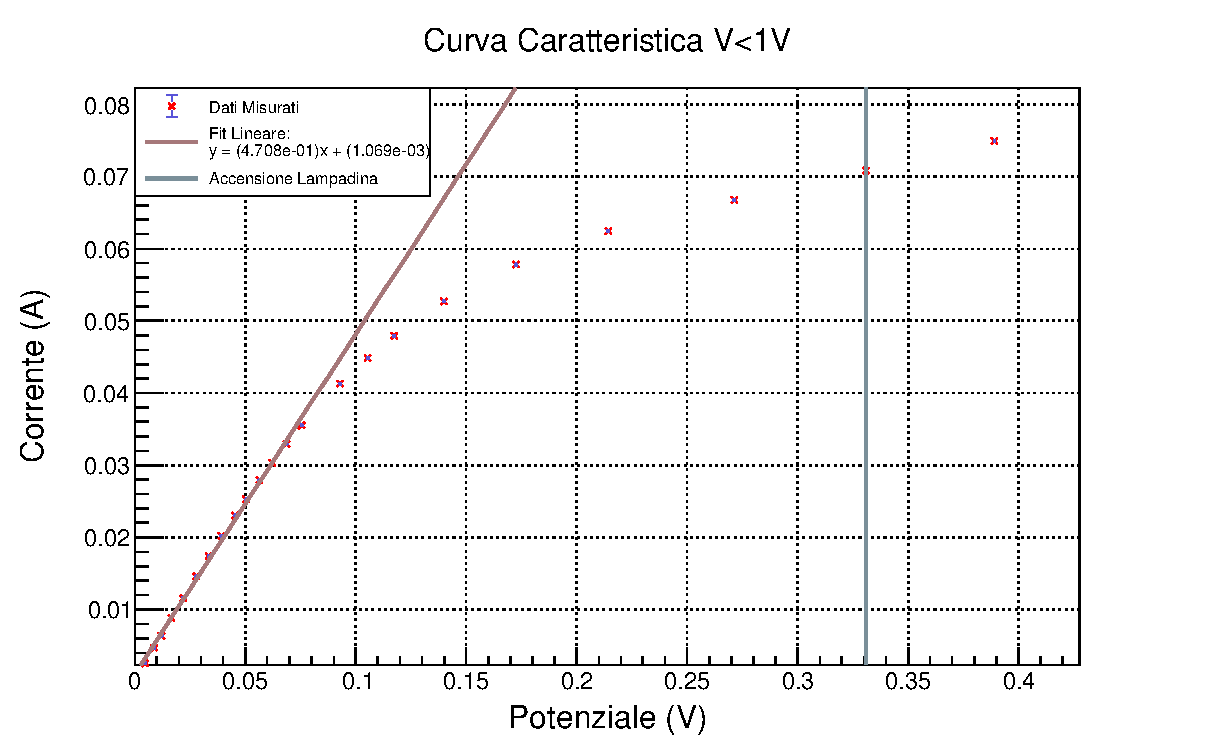
\includegraphics[width=0.9\textwidth]{immagini/graficozoomato1.eps}
        \caption{Grafico fino all'accensione della lampadina}
\end{figure}
\FloatBarrier
\noindent{Infatti, con l'aumento della temperatura aumenta la resistività del materiale e quindi aumenta di conseguenza la resistenza, deviando dal comportamento lineare.}

Misurando nello stesso tempo la corrente emessa dal fotodiodo, è stato registrato un valore circa costante di $I=0.15$mA dall'accensione dell'alimentatore. Per $V=0.3310$V è stato misurato un'aumento netto di corrente $I=0.50$mA corrispondente alla prima transizione di fase: la lampadina inizia ad emettere luce oltre al riscaldamento per effetto Joule. 

Da $V=0.520$V la corrente emessa dal fotodiodo inizia ad assumere valori anomali. Questo potrebbe essere causato dalla saturazione del fotodiodo. Per questo motivo, si è passati alla seconda fase dell'esperimento, togliendo il fotodiodo e la resistenza dal circuito: il fotodiodo serviva solo a registrare l'istante di accensione della lampadina. 

\begin{figure}[!htbp]
  \centering
      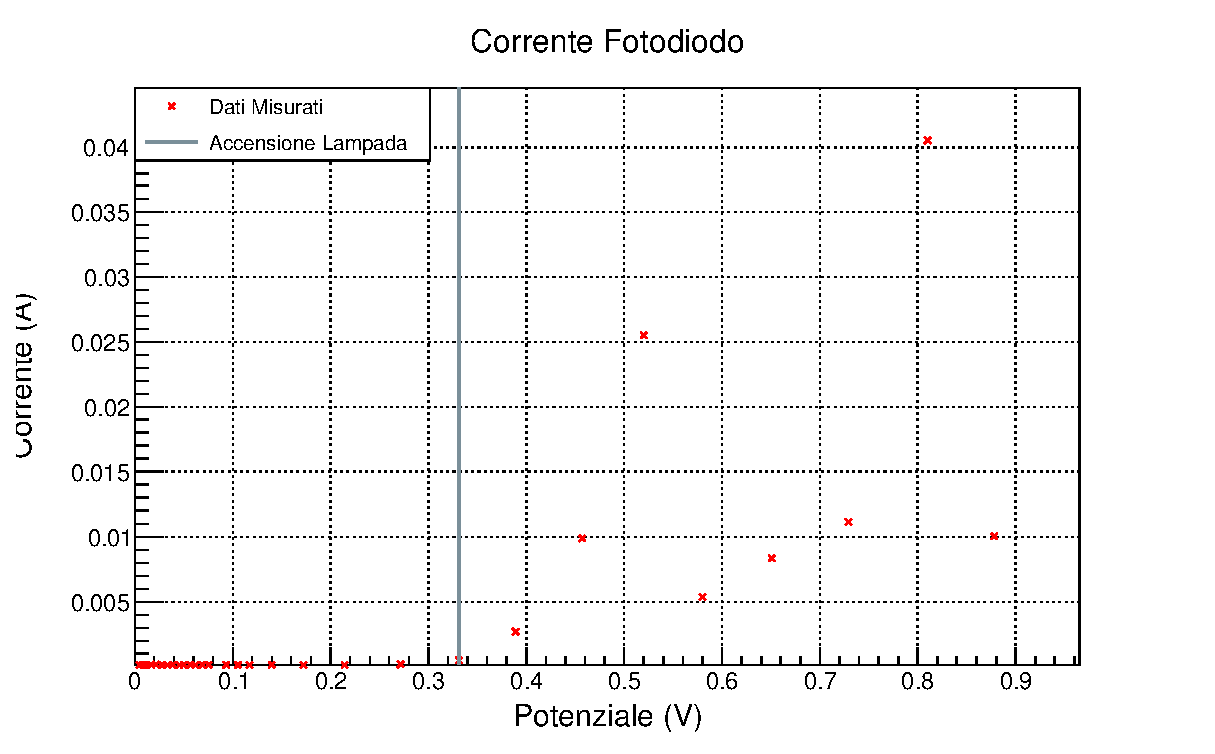
\includegraphics[width=0.9\textwidth]{immagini/fotodiodografico.eps}
        \caption{Andamento della corrente emessa dal fotodiodo in funzione del potenziale erogato dall'alimentatore}
\end{figure}
\FloatBarrier

Valutando la proporzionalità tra il potenziale e la corrente in seguito all'accensione della lampadina, si è ottenuto un andamento lineare graficando sulle ascisse il potenziale e sulle ordinate la corrente al quadrato, ottenendo così m = $(1.58\pm0.02) \times 10^4$ mA$^2$/V e q = (-4 $\pm 1) \times 10^3$ mA$^2$. Si ottiene così la seguente proporzionalità: $I\propto \sqrt{V}$.

In questo caso, l'alta percentuale di incertezza è dovuta alla scelta di usare come errore su $I^2$ la media aritmetica degli errori ($\pm 3.167$V) per il metodo dei minimi quadrati. 

\begin{figure}[!htbp]
  \centering
      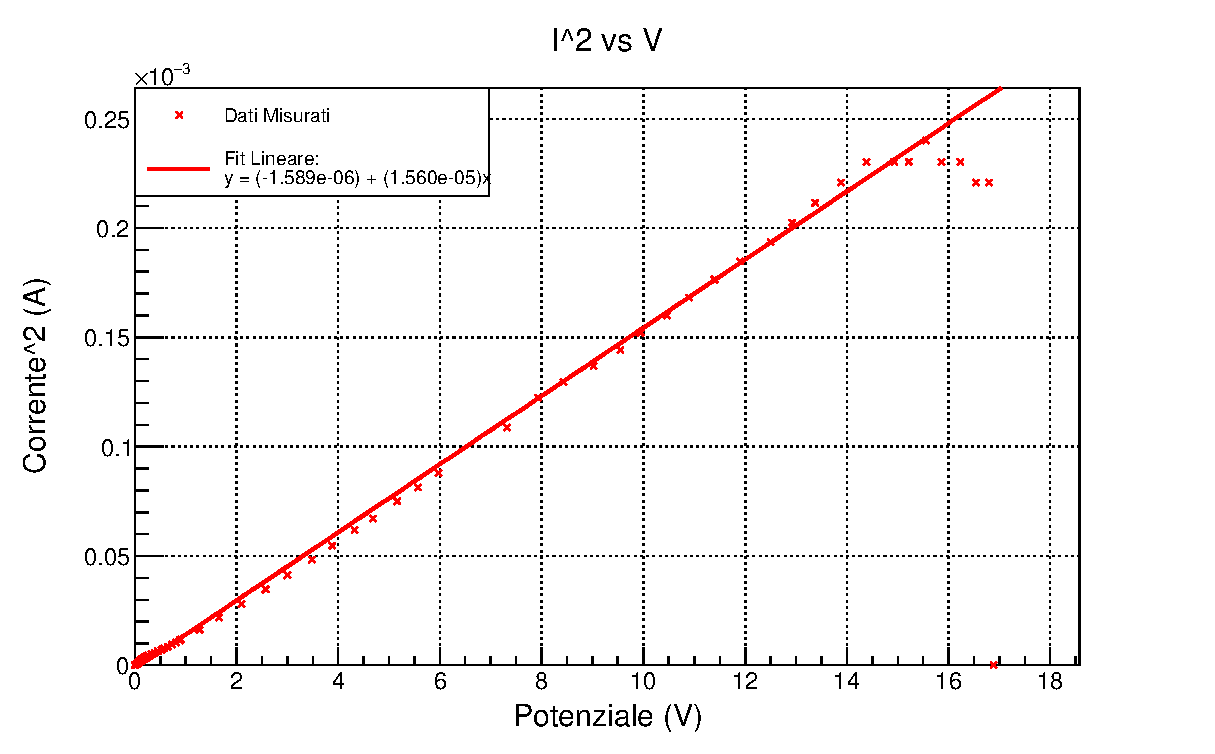
\includegraphics[width=0.9\textwidth]{immagini/I2vsV.eps}
        \caption{Curva caratteristica scala semi-quadratica}
\end{figure}
\FloatBarrier

Dal momento che la resistenza della lampadina non segue un andamento ohmico, è utile definire la resistenza dinamica su intervalli i-esimi: $R_{i} = \frac{\Delta V_i}{\Delta I_i}$. 

Graficando la resistenza dinamica così calcolata in funzione del potenziale, si vedono il cambio di pendenza e le fluttuazioni corrispondenti alle due transizioni di fase. In particolare, nella seconda si ottengono valori della resistenza dinamica molti diversi tra loro e addirittura in certi casi negativi. 

\begin{figure}[!htbp]
  \centering
      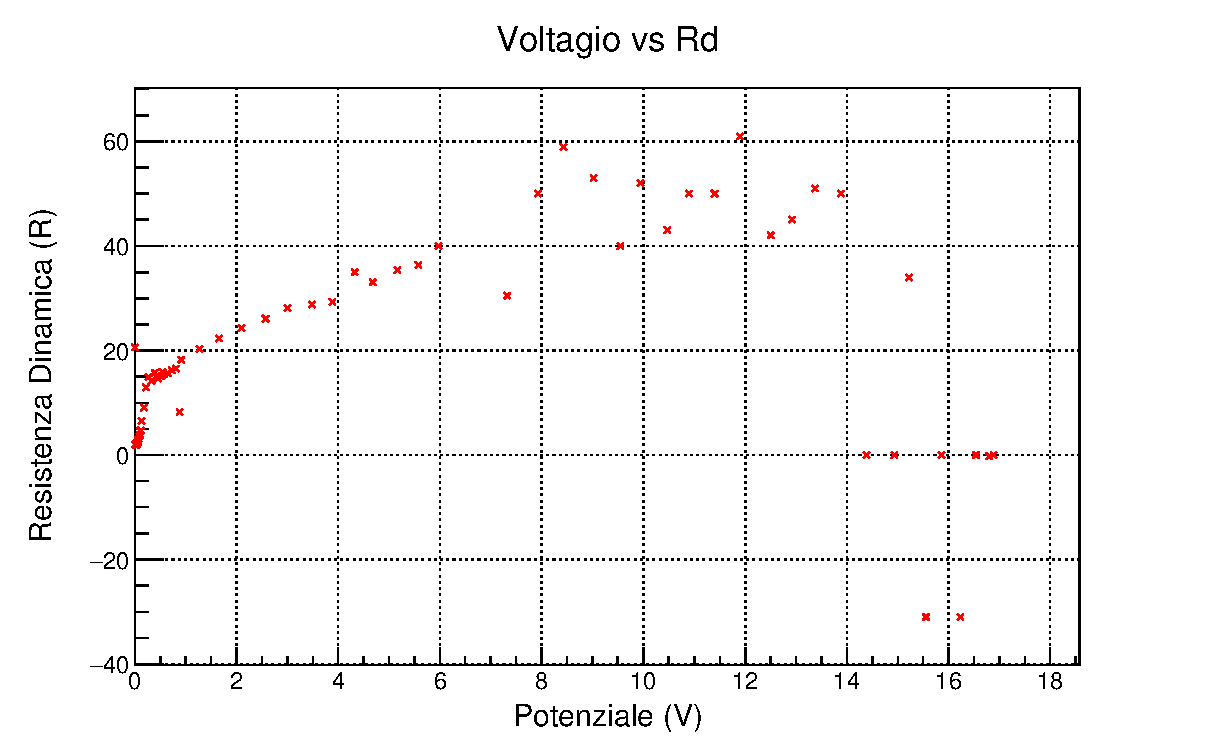
\includegraphics[width=0.9\textwidth]{immagini/fotodiodord.eps}
        \caption{Resistenza dinamica in funzione del potenziale}
\end{figure}
\FloatBarrier

\noindent{Questo può essere spiegato dal filamento che inizia a bruciare e poi sciogliere, creando anche bolle di gas metallico all'interno di esso, fino al completo scollegamento del filamento stesso, e quindi del circuito. Ciò può essere anche constatato osservando il bulbo della lampadina, che presenta un completo annerimento causato dal vapore metallico.}

In questo grafico, le barre d'errore sull'asse y, non sono state indicate dopo $V = 7.93$V perché la minima variazione della corrente portava ad avere un'incertezza relativa elevata, che avrebbe reso il grafico illegibile. 

\section{Conclusione}
Gli errori associati alle misure dovuti alla sensibilità degli strumenti non compaiono in maniera apprezzabile sui grafici, fatta eccezione per le grandezze derivate. Una possibile fonte d'errore sistematico potrebbe essere il cambiamento della scala dei multimetri una volta raggiunto il fondoscala: ciò potrebbe aver aumentato o diminuito i valori effettivi. 

Il comportamento anomalo del fotodiodo osservato in questa istanza richiede una migliore analisi. 

Per quanto riguarda l'ambito di interesse di questo esperimento, la curva caratteristica della lampadina ottenuta è conforme a quanto aspettato.
\end{document}